We use a demo application, accessible with a web browser, to present the working prototype.
It can be used to find sentence boundaries in unpunctuated text.
The general web page shows two main tabs, one labeled \emph{Lexical} and one \emph{Lexical + Audio}.
A user can click these, to switch between using only the lexical model or the fusion of both the lexical and the acoustic model.

There are two ways to feed input to our model for the \emph{Lexical} SBD (see Figure~\ref{fig:demo_l}).
\begin{figure}[ht]
    \centering
    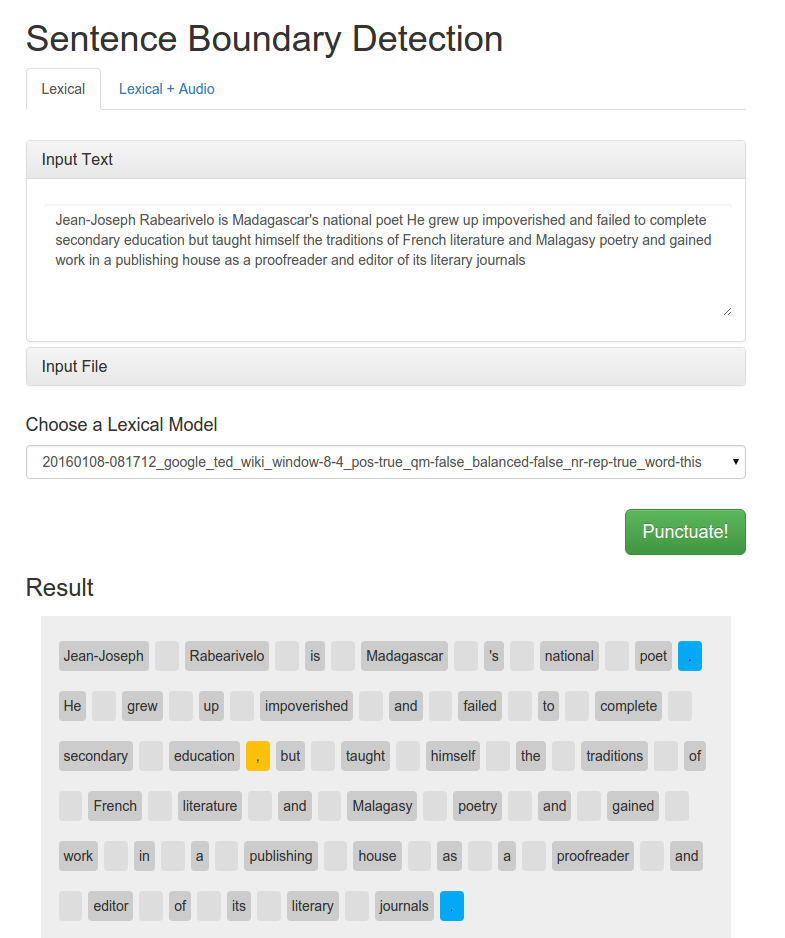
\includegraphics[width=0.5\textwidth]{img/demo_l.png}
    \caption{The demo application for lexical model. The results are presented below the options for input and model selection.}
    \label{fig:demo_l}
\end{figure}
The user can enter a text input field to manually enter or paste any text they wish.
Another possibility is to choose from a set of existing text files.
A dropdown selection allows the user to choose the pretrained models, if multiple models are available in the system.
If the model is changed, it is automatically loaded in the background.
Once the user clicks the \emph{Punctuate!} button, the text, which was entered, or selected as a file, is passed to our lexical model.
While the server processes the request, a small loading icon is shown inside the button.
After the predictions are returned from the server, the result is shown beneath.
The input text and positions where no punctuation was predicted are shown as tokens with a light grey background.
Any commas or periods inserted, are shown in distinct colors.
If a model, which uses POS tags, is selected a user can hover their mouse over a token to see its POS category.
For further use the entire result is selectable and can be copied.

For the \emph{Lexical + Audio} SBD the possibilities for entering input are more limited (see Figure~\ref{fig:demo_la}).
\begin{figure}[ht]
    \centering
    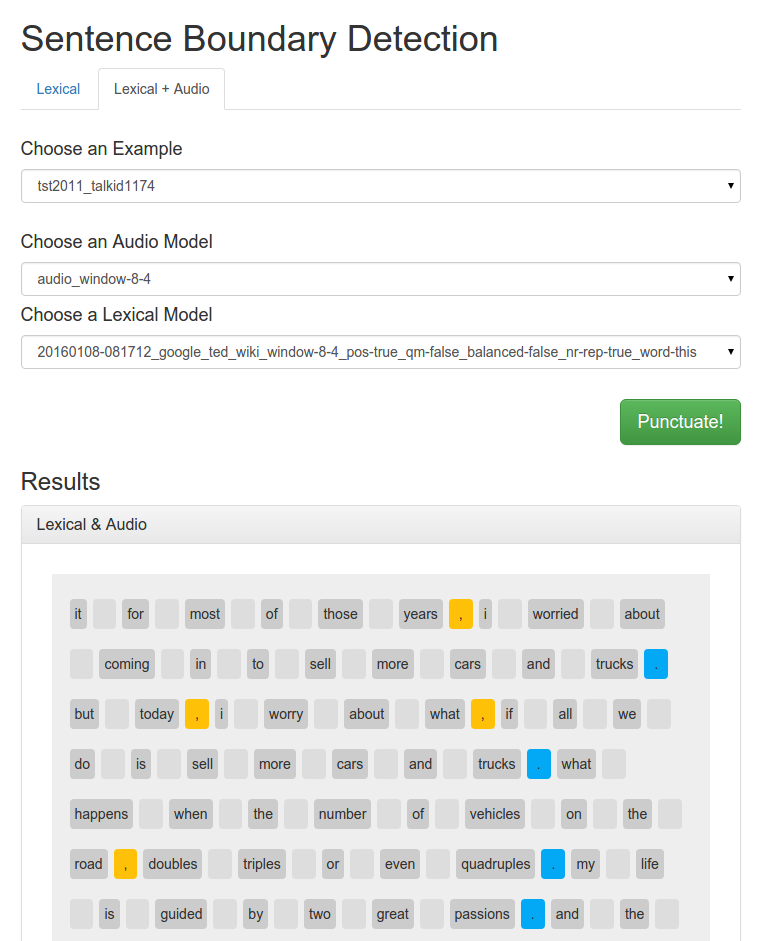
\includegraphics[width=0.5\textwidth]{img/demo_l_a.png}
    \caption{The demo application for fusion of both models. The results of the individual models and the fusion are presented below the options for input and model selection. Only one result section is in the screenshot, the other sections are out of the region of the screenshot.}
    \label{fig:demo_la}
\end{figure}
Since we need an audio recording, we offer only examples existing in the system.
At the moment the system contains samples, which were used in the testing phase, but not for training.
The selection of the user is therefore limited by a dropdown menu of all available choices.
However, the choice of both the acoustic and the lexical model is independently available to a user.
These can also be selected in a dropdown menu.
The functionality of the \emph{Punctuate!} button is unchanged.
It triggers the processing and shows a loading indicator until the result returns.
The result area however is changed, and contains three subareas, which each contain a different result.
Two of them contain the raw results of the acoustic model and the lexical model.
The third shows the result after the fusion.
Therefore, it is easy to compare the results of each individual model, and the result after the fusion.
